\documentclass[10pt,a4paper,onecolumn]{article}
\usepackage[left=0.75in, right=0.75in, top=1.00in, bottom=1.00in]{geometry}
\usepackage{url}
\usepackage[parfill]{parskip}
\usepackage{xcolor,colortbl}
\usepackage{hyperref}
\hypersetup{colorlinks=true,
linkcolor=red}
\usepackage{graphicx}
\definecolor{Gray}{gray}{0.85}
\usepackage{tabularx}
\usepackage{float}
\usepackage{multirow}

%opening
\title{Political Ideology Bias Detection with BERT}
\author{Ahsen Qamar and Alex Dauenhauer}

\begin{document}

\maketitle

\begin{abstract}
In this paper, we attempt to use Google's recently released BERT model to detect political ideology bias at the sentence level. We use a pre-processed dataset from the Ideological Books Corpus (IBC) \cite{iyyerRNN} as well as adapting a method of filtering and labeling from Iyyer et al. \cite{iyyerRNN} to generate two new datasets from raw document corpora, the Convote dataset \cite{convote} and the All-the-news dataset \cite{news}. We perform experiments using a "train on one, test on all" format. Our model performs well when evaluated on the same set it was trained with, and shows that there is room for improvement in being able to generalize from one dataset to the other. Our model achieves F1-scores of 99.4\% when trained and tested with our All-the-news dataset, 92.6\% with the Convote dataset and 56.8\% with the IBC dataset. For document level bias detection, we achieve an F1-score of 60\% on the Convote dataset and 50\% on the All-the-news dataset.
\end{abstract}

\section{Introduction}
\label{intro}
Political ideology bias in news sources is a topic of growing concern, not just in the U.S., but across the entire world. As our country grows ever more partisan and misinformation campaigns fuel distrust in mainstream news sources, people have a tendency to turn to alternative news sources which typically reflect the existing ideology bias of the author. This creates echo chambers and reinforces existing partisan ideologies driving the partisan divide ever wider. The ability to automatically label biased text could inform readers that may have otherwise assumed the content was neutral, and encourage them to pursue alternative sources with less bias, or at the very least maintain a degree of skepticism about the content they are consuming. A system like this could also help media sources reduce the amount of bias they include their reporting, some of which may be unconscious and therefore undetected by writers or editors. Using this tool as a proofreader of sorts could eventually, hopefully reduce the amount of bias in media and reduce the growing partisan divide.

In this paper, we build off of previous work done by Iyyer et al. \cite{iyyerRNN}. Their success in using an RNN model to predict ideological bias at the sentence level, inspired us to expand on their experiments using BERT \cite{bert}, a modern transformer-based model that achieves state-of-the-art results\footnote{At the time this sentence was written} on a number of different NLP problems. We use a BERT implementation for sequence classification to predict ideological bias at the sentence level on three unique datasets. We use a processed subset of sentences from the Ideological Books Corpus (IBC) \cite{gross2013ibc}. We also use a filtering method explained in section \ref{sec:filtering} to select a set of biased sentences from the Convote dataset \cite{convote}. Additionally, we build a new dataset by filtering a corpus of news articles from 15 different publishers \cite{news}, with bias labels sourced from mediabiasfactcheck.com (MBFC) \cite{mbfc}. We predict bias at the sentence level, then use the aggregate sentence level predictions to predict bias at a document level and compare to the publisher label assigned by the MBFC team. which  described in greater detail in section \ref{sec:data}

\section{Model \& Architecture}
BERT (Bidirectional Encoder Representations from Transformers) was released late last year by Google. The main draw towards the use of BERT for this project was leveraging the bi-directional training transformer to help detect political bias in text. For more information regarding BERT please refer to this \href{https://arxiv.org/abs/1810.04805}{research paper} from Google.

A cloud instance hosting an Nvidia P100 GPU was our environment for hosting our data as well as deploying our model for training and evaluation. This infrastructure limited us to use the BERT \textit{base} models as the GPU would continually run out of memory with the slightly larger models. No significant difference was found between \textit{cased} and \textit{uncased} for the \textit{base} models so we decided to move forward with \textit{BERT-Base, Cased}. The decision was made to move forward with a \textbf{pytorch} backend due to more thorough availability of code examples and better documentation. The primary reference for our code was from a \textit{Medium} article \cite{usingbert}. A high level diagram of our overall architecture is shown in Figure \ref{fig:architecture}:
\begin{figure}[h]
	\begin{center}
		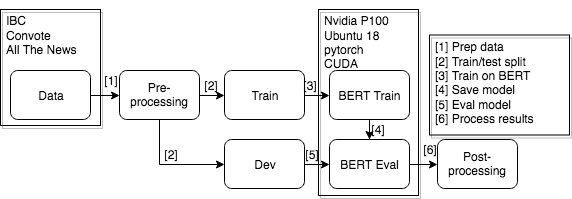
\includegraphics[width=0.8\linewidth]{architecture.png}
		\caption{Architecture}
		\label{fig:architecture}
	\end{center}
\end{figure}
Data was obtained from three different sources and funneled into a pre-processing step. This involved generating sentences with labels of liberal, neutral, or conservative and formatting the data into a tsv that BERT would accept. We then perform a random 70:30 train/dev split. Train data is fed into our BERT train script and the generated model is saved and funneled into our BERT eval script. The model is then evaluated on the dev data. An averaging classification layer is added as part of post-processing for documents. Let's take a look at what all is moving through our pipeline. 

\section{Data}
\label{sec:data}
Political bias at the sentence level is a very subjective topic and therefore, there are not many large corpora widely available for use. A large part of this project was devoted to acquiring and preparing a few existing corpora, as well as repurposing a few processing methods on new corpora to develop our own biased sentence corpus. We performed experiments on three separate datasets: the Ideological Books Corpus (IBC) \cite{iyyerRNN}, Annotated congressional floor debates \cite{convote}, and the all-the-news dataset from Kaggle user Andrew Thompson \cite{news}. In this section we will describe the content of each dataset and processing steps performed on each dataset for use in our model.

\subsection{IBC}
The Ideological Books Corpus was provided to us in a fully processed format, courtesy of Iyyer et al.\cite{iyyerRNN} The original IBC dataset, developed by Gross et al.\cite{gross2013ibc} is a collection of books and articles written between 2008 and 2012 by well-known authors with strong political leanings. What Iyyer et al. did was to filter this corpus using a similar strategy to our strategy outlined in section \ref{sec:filtering}\footnote{Iyyer's team used bigrams and unigrams as their bias detectors, whereas we use trigrams and bigrams}. They then crowd-sourced manual ideological bias annotations of the resulting sentences and particular subphrases. We use the data in this processed form as is, with no further processing. This provides a more subjective approach to bias labeling which we can compare with our objective labeling approach described in section \ref{sec:filtering}

\subsection{Convote}
The Convote dataset is a corpus of congressional speeches with each speech treated as a document with automatically derived labels of the speaker's political party (D, for Democrat; R, for Republican; I for Independent) as well as other related extracted information that was not pertinent to our experiments. Since our work attempts to predict ideological bias rather than political party, we relabel each document by mapping Democrat to "liberal", Republican to "conservative" and Independent to "neutral"\footnote{While we realize that a politician of Independent party certainly does not imply that politician's dialogue will contain no ideological bias, we use this label to select sentences that contain no bias detectors from either the liberal or conservative ideology which is explained further in section \ref{sec:filtering}.}. While it is true that the mapping of political party directly to political bias is not always a 1:1 relationship, there is a strong correlation between political party and political ideology. Further, we expect that our method for filtering the dataset (explained in section \ref{sec:filtering}) for biased sentences will wash out noise that would be seen from speeches made by moderate centrists on either side of the aisle.

\subsection{All-the-news Kaggle corpus}
To expand our training data further with a greater diversity of authors, we turned to a Kaggle corpus of 142,570 news articles from 15 different publishers as provided by Andrew Thompson \cite{news}. We assigned each publisher a bias label, sourced from mediabiasfactcheck.com (MBFC), then we simplified these labels down to the same labels we used in the previous datasets: liberal, conservative and neutral. The labels assigned to each publisher are shown in Table \ref{tab:pub-bias}.

\begin{table}[h!]
	\begin{center}
		\caption{Publisher and bias labels from all-the-news corpus}
		\label{tab:pub-bias}
		\begin{tabular}{c|c|c}
			\hline\hline
			\textbf{Publisher} & \textbf{MBFC Bias Label} & \textbf{Simplified Bias Label} \\
			\hline
			New York Times & left-center & liberal \\
			\rowcolor{Gray}
			Breitbart & extreme-right & conservative \\
			\rowcolor{Gray}
			CNN & left & liberal \\
			Business Insider & left-center & liberal \\
			Atlantic & left-center & liberal \\
			\rowcolor{Gray}
			Fox News & right & conservative \\
			\rowcolor{Gray}
			Talking Points Memo & left & liberal \\
			Buzzfeed News & left-center & liberal \\
			National Review & right & conservative \\
			New York Post & right-center & conservative \\
			Guardian & left-center & liberal \\
			NPR & left-center & liberal \\
			Reuters & neutral & neutral \\
			\rowcolor{Gray}
			Vox & left & liberal \\
			Washington Post & left-center & liberal \\
			\hline\hline
		\end{tabular}
	\end{center}
\end{table}

\subsection{Biased Sentence Selection}
\label{sec:filtering}
It would be extremely unreasonable to assume that every sentence spoken by a member of congress during a congressional debate would contain ideological bias. Or that every sentence written by every author published under a specific news publisher would contain the bias of that publisher. In fact, a large portion of the sentences in both the Convote dataset and the All-the-news dataset contain no bias at all. Therefore, it is necessary to filter these datasets for sentences that explicitly contain bias, prior to labeling those sentences and using them to train our model.

To select the explicitly biased sentences from the data, we used a method inspired by Yano, et al. \cite{YanoBigrams} and similar to a method used by by Iyyer, et al \cite{iyyerRNN} that was shown to be successful at identifying bias indicators. We started by identifying the most frequently used trigrams and bigrams for each bias label, liberal or conservative (in the Convote set, we used the full corpus to identify n-grams, whereas in the All-the-news data, we use a subset of the publishers with the most extreme MBFC bias labels to identify n-grams. This subset of publishers is highlighted in gray in Table \ref{tab:pub-bias}). We then filtered out any trigrams or bigrams which contained stopwords, and English names\footnote{Removing stopwords serves the purpose of eliminating trigrams and bigrams that contain commonly used words, but don't contain substance for bias. Removing English names was a strategy that proved effective in filtering the All-the-news dataset (removing references to prolific journalists or prominent politicians), and was applied to the Convote data as well, essentially serving the purpose of removing n-grams that are sourced from replies to other speakers that address the other speaker by name}. We further filtered each bigram list by requiring that at least one word in each bigram contain an "opinion" word, defined as a word found in the \texttt{opinion\_lexicon} corpus from NLTK\footnote{This strategy intends to select only those phrases that contain an ideological opinion which would typically be seen as a strong indicator of bias, when spoken by someone with known political affiliation. We decided to not make this a requirement for the trigrams as we felt these phrases would be unique enough to each ideology without this additional criteria that we did not want to lose information by filtering too heavily.}. We then took the set difference of the resulting top 1000 most frequent liberal and conservative n-grams. We kept the top 100 filtered bigrams and top 100 filtered trigrams for each label as our bias indicators (for a total of 200 bias indicators for each label). We then filtered sentences such that, if a democratic speaker (or author from a liberal publisher) spoke a sentence that contained one of these top 200 liberal bias indicators, we labeled that sentence as "liberal" and used the same logic for republican speakers/conservative publishers to identify "conservative" sentences. For these datasets, we identified a neutral sentence as one which was spoken by an independent politician or neutral publisher\footnote{Reuters is the only publisher labeled as "neutral" by MBFC} and contained no n-grams from either the liberal or conservative bias indicator lists. The top 10 bias indicators from each label for the Convote data are shown in Table \ref{tab:ngrams-convote} and those from the All-the-news data are shown in Table \ref{tab:ngrams-atn}. The resulting Convote dataset included 1326 conservative sentences, 1383 liberal sentences and 213 neutral sentences. The resulting All-the-news dataset contained 16,745 conservative sentences, 28,230 liberal sentences, 277,751 neutral sentences. To balance this dataset and avoid weighting strategies while training, we pared this down to a random selection of 16,000 sentences from each label, for a total of 48,000 sentences. Example sentences from each ideology label for the Convote data are shown in Table \ref{tab:convote-sentences} and examples from the All-the-news data are shown in Table \ref{tab:atn-sentences}.

\begin{table}[h!]
	\begin{center}
		\caption{Top 10 n-grams per ideology label - Convote}
		\label{tab:ngrams-convote}
		\begin{tabular}{p{0.22\linewidth}|p{0.22\linewidth}|p{0.22\linewidth}|p{0.22\linewidth}}
			\hline\hline
			\multicolumn{2}{c|}{\textbf{Liberal}} & \multicolumn{2}{c|}{\textbf{Conservative}} \\
			\hline
			\multicolumn{1}{c|}{Trigrams} & \multicolumn{1}{c|}{Bigrams} & \multicolumn{1}{c|}{Trigrams} & \multicolumn{1}{c|}{Bigrams} \\
			\hline
			social security trust & tax breaks & national electrical contractors & community protection \\
			security trust fund & security trust & electrical contractors association & free market \\
			cbc alternative budget & bad policy & legislative days within & organized crime \\
			black caucus budget & would lose & inner cell mass & bankruptcy relief \\
			estate tax relief & reduce crime & head start program & good news \\
			privatize social security & budget reconciliation & community protection act & relief extension \\
			u.s. trade deficit & ethical standard & million new jobs & delayed notification \\
			republican budget resolution & fiscally irresponsible & death tax repeal & soft money \\
			national wildlife refuge & working poor & 9/11 commission report & illegal aliens \\
			guardian ad litem & subpoena power & stem cells without & invasive species \\
			\hline\hline
		\end{tabular}
	\end{center}
\end{table}

\begin{table}[h!]
	\begin{center}
		\caption{Sample sentences from each ideology label - Convote}
		\label{tab:convote-sentences}
		\begin{tabular}{p{0.3\linewidth}|p{0.3\linewidth}|p{0.3\linewidth}}
			\hline\hline
			\multicolumn{1}{c|}{\textbf{Liberal}} & \multicolumn{1}{c|}{\textbf{Conservative}} & \multicolumn{1}{c|}{\textbf{Neutral}}\\
			\hline
			mr. speaker, during a time of war, in the aftermath of a catastrophic hurricane, with 45 million americans lacking health insurance and skyrocketing home heating costs projected this winter, this majority is proposing to take from those with the least, give to those with the most -- and tell our children they will have to pay for it all later. & on both the business records and delayed notification sections of the patriot act (among others), the stance of the american civil liberties union and like-minded critics seems to have an ulterior motive. & let us look at what is going on in america today. \\
			it is clear that there would be plenty of money to deal with the social security trust fund if the president were not using the social security trust fund as a slush fund to give tax cuts to the wealthiest people in america. & that legislation helped to streamline the intelligence community and tightened some asylum rules that allowed potential terrorists to remain in our country. & mr. speaker, parliamentary inquiry. \\
			\hline\hline
		\end{tabular}
	\end{center}
\end{table}

\begin{table}[h!]
	\begin{center}
		\caption{Top 10 n-grams per ideology label - All-the-news}
		\label{tab:ngrams-atn}
		\begin{tabular}{p{0.22\linewidth}|p{0.22\linewidth}|p{0.22\linewidth}|p{0.22\linewidth}}
			\hline\hline
			\multicolumn{2}{c|}{\textbf{Liberal}} & \multicolumn{2}{c|}{\textbf{Conservative}} \\
			\hline
			\multicolumn{1}{c|}{Trigrams} & \multicolumn{1}{c|}{Bigrams} & \multicolumn{1}{c|}{Trigrams} & \multicolumn{1}{c|}{Bigrams} \\
			\hline
			senior administration official & opioid epidemic & jerusalem bureau chief & illegal aliens \\
			greenhouse gas emissions & health reform & border patrol agent & illegal alien \\
			north korean leader & lethal injection & social justice warriors & illegal immigrant \\
			federal civil rights & healthy people & black panther party & migrant crisis \\
			provocative narrative essays & racial bias & cartel chronicles project & patriot channel \\
			clean air act & budget reconciliation & refugee resettlement program & hard truths \\
			health care policy & chronic pain & prison sentence commuted & twin falls \\
			republican health care & lead poisoning & god less america & islamic terror \\
			gop health care & intelligence committees & real clear politics & snarky opinions \\
			civil rights laws & rights advocates & face certain death & dangerous faggot\footnotemark \\
			\hline\hline
		\end{tabular}
	\end{center}
\end{table}
\footnotetext{The extreme offensiveness of this bigram led us to investigate its origins further. The presence of this bigram is not actually due to conservative media using slurs like this commonly enough to rank in our top ten list. Instead it is actually a reference to "The Dangerous Faggot Tour" which is a campus speaking tour of Milo Yiannopoulos, a prominent contributor to Breitbart News. This is not to condone the use of this offensive slur, just to explain its origins and presence in this list a bit more clearly}

\begin{table}[h!]
	\begin{center}
		\caption{Sample sentences from each ideology label - All-the-news	}
		\label{tab:atn-sentences}
		\begin{tabular}{p{0.3\linewidth}|p{0.3\linewidth}|p{0.3\linewidth}}
			\hline\hline
			\multicolumn{1}{c|}{\textbf{Liberal}} & \multicolumn{1}{c|}{\textbf{Conservative}} & \multicolumn{1}{c|}{\textbf{Neutral}}\\
			\hline
			Here’s what you need to know: American divisions are rapidly widening over President Trump’s order to close the U. S. to refugees and people from seven predominantly Muslim countries. & And the costs of illegal alien crime continued to mount and a lethal opioid epidemic raged. & Showcasing their attempts to unite with other groups for the election, Islamists campaigned with Awdeh Qawwas, a prominent priest, in the affluent Abdoun district of the capital Amman. \\
			In a video posted on her campaign’s Facebook page shortly after Mr. Sanders departed the White House grounds to visit the Capitol, Mr. Obama described Mrs. Clinton as the most qualified candidate to seek the White House, and implored Democrats to come together to elect her after a divisive party primary. & Obama’s claim of civic peace is also at odds with the televised evidence: dramatic race riots, cop killings, rapes, murders, illegal alien crimes, and chaos that rippled across the country during the second term of his presidency. & Rousseff’s survival hinges on winning over a dwindling number of undecided lawmakers who are also being courted by the man poised to take over if she is ousted, Vice President Michel Temer. \\
			\hline\hline
		\end{tabular}
	\end{center}
\end{table}

\section{Experiments/Results}
When experimenting with BERT we found the following configuration of BERT parameters to provide the best results: $MAX\_SEQ\_LEN = 256$, $TRAIN\_BATCH\_SIZE = 16$, $LEARNING\_RATE = 2e-6$, \newline
$NUM\_TRAIN\_EPOCHS = 3$. The $MAX\_SEQ\_LEN$ and $TRAIN\_BATCH\_SIZE$ are the maximum possible values selected given we were using an Nvidia P100 and concurrently dependent on our Cuda version. The $LEARNING\_RATE$ is the default provided by BERT. $NUM\_TRAIN\_EPOCHS$ was set to 3 after continuous experimentation and analysis of the evaluation loss which saturated after about 2.5 epochs. These parameters remained the same for all three datasets.

As seen in Table \ref{tab:res-mat}, the \textit{IBC} dataset had the worst performance both on itself as well as the other datasets. The evaluation accuracy is highest on itself, followed by \textit{AllTheNews} with an accuracy of 40\%, and then \textit{Convote} with an accuracy of 40\%. What is surprising is that f1 scores are higher than accuracy on all the datasets besides itself. The evaluation loss saturated at 0.99 (Table \ref{tab:eval-loss}) hinting at the fact that the dataset is fairly small.

The \textit{Convote} had fairly good performance with an evaluation accuracy of 91\% on itself. It had an accuracy of 63.5\% on \textit{AllTheNews} which is significantly better than \textit{IBC}. Lowest evaluation accuracy was on \textit{IBC} at 20\%. F1 scores very closely mirrored their respective accuracies. The evaluation loss improved when compared to \textit{IBC} at 0.23. Again, the evaluation loss saturated and despite having more data than \textit{IBC} we still might not have enough.

The best performance of all the datasets was from \textit{AllTheNews} with an evaluation accuracy of 99.4\% on itself. It had a similar evaluation accuracy on \textit{IBC} to that of \textit{Convote}. On the \textit{Convote} dataset it obtained an evaluation accuracy of 60\%. The f1 scores were lower on the \textit{IBC} and \textit{Convote} when compared to the evaluation accuracies. We saw the lowest evaluation loss at 0.02 which is significantly better than any of the other datasets.

\begin{table}[H]
\centering
\caption{Results Matrix}
\label{tab:res-mat}
\begin{tabular}{p{0.15\linewidth}||p{0.08\linewidth}|p{0.08\linewidth}|p{0.08\linewidth}|p{0.08\linewidth}|p{0.08\linewidth}|p{0.08\linewidth}|p{0.08\linewidth}|p{0.08\linewidth}}
 \hline
  \multirow{2}{*}{\textbf{Train/Test}} & \multicolumn{2}{c|}{\textbf{IBC}} & \multicolumn{2}{c|}{\textbf{Convote}} & \multicolumn{2}{c|}{\textbf{AllTheNews}} & \multicolumn{2}{c}{\textbf{Documents}} \\ 
  \cline{2-9}
  & \footnotesize{\textbf{Accuracy}} & \footnotesize{\textbf{F1-score}} & \footnotesize{\textbf{Accuracy}} & \footnotesize{\textbf{F1-score}} & \footnotesize{\textbf{Accuracy}} & \footnotesize{\textbf{F1-score}} & \footnotesize{\textbf{Accuracy}} & \footnotesize{\textbf{F1-score}} \\
 \hline\hline
 \textbf{IBC} & \centering 60\% & \centering 56.8\% & \centering 22.8\% & \centering 28.6\% & \centering 40\% & \centering 49\% & \centering N/A & \multicolumn{1}{c}{N/A} \\ 
 \textbf{Convote} & \centering 20\% & \centering 16.8\% & \centering 91\% & \centering 92.6\% & \centering 63.5\% & \centering 63.4\% & \centering 61.18\% & \multicolumn{1}{c}{60\%} \\ 
 \textbf{AllTheNews} & \centering 16.8\% & \centering 10.5\% & \centering 60\% & \centering 49.1\% & \centering 99.4\% & \centering 99.4\% & \centering 65\% & \multicolumn{1}{c}{50\%} \\ %[1ex]
 \hline
\end{tabular}
\label{table:results}
\end{table}

\begin{table}[h!]
\centering
\caption{Evaluation loss}
\label{tab:eval-loss}
\begin{tabular}{c|c|c} 
 \hline\hline
 \textbf{IBC} & \textbf{Convote} & \textbf{AllTheNews} \\ [0.5ex] 
 \hline
 0.99 & 0.23 & 0.02 \\ [1ex]
 \hline\hline
\end{tabular}
\end{table}

\section{Conclusion}
\subsection{Bias labeling at phrase level}
The n-gram filtering task shed light on how each ideology uses different, yet equally charged phrases to describe the same term. For example, one of the top liberal trigrams in the Convote dataset was "estate tax relief" whereas a top conservative trigram was "death tax repeal", where both are referring to the same topic. Another example, in the all-the-news dataset, a top conservative bigram is "illegal immigrants" with the liberal equivalent being "undocumented immigrants"\footnote{This was one of the top bigrams in content labeled "liberal", however, neither the word \textit{undocumented}, nor the word \textit{immigrants} are an opinion lexicon and therefore our final filtering strategy removes this bigram as a bias detector. In future work, we would like to determine a more sophisticated n-gram detection method}. In the Convote and All-the-news datasets, we used the presence or absence of an n-gram bias phrase in a sentence to label the ideology bias at the sentence level. This provides an objective methodology for bias labeling, rather than a subjective system, which would be heavily dependent on the reader's own personal biases. The IBC corpus relies on a subjective (human-determined) labeling methodology\footnote{While the crowd-sourced nature of the labeling of this corpus removes some measure of subjectivity, the labels are still based on human opinions of whether a sentence is biased or not.}. 

\subsection{Bias detection at sentence level} 
The first and foremost conclusion we can draw from experiments to detect bias at the sentence level is that our model performs well when evaluated using a test set from the corpus with which it was trained (the diagonal of Table \ref{table:results}), but it is not generalizing well enough to handle the variation in language style that exists between our datasets. For example, when we train the model with the all-the-news corpus, we achieve an F1-score of 99.4\% when using a test set from the same corpus, but testing on the IBC corpus gives an abysmal F1-score of 10.5\%. Training on the IBC corpus (which consists of sentences extracted from books written by prominent authors with known ideological bias) performs terribly on the Convote corpus, and is no better than a coin toss on the all-the-news corpus. This isn't completely surprising since there are great differences between the language used during a parliamentary speech and the language used in an ideological book (which may be trying to persuade its reader to believe a certain idea), which is in turn very different from the language used in a news article (which has limited words to convey its message and in theory should be trying to present the facts of an event, rather than opinions about an event).

The drop in performance we see with the IBC dataset as compared to the Convote and All-the-news datasets is likely explained by greater variation in sentence content, relative to the size of the dataset. The IBC dataset is labeled in a subjectively (by humans) rather than the objective labeling method we applied to the Convote and All-the-news data. This allows for a much broader interpretation of what content would consitute bias. In the objective case, the sentence is required to contain one or more n-grams from a curated list to be labeled as biased which restricts the allowable content and subject matter of the sentence. In the subjective case, there is no such requirement and the human labels the bias of the sentence based on their own judgement\footnote{Iyyer et al. also used a similar n-gram filtering method to select sentences that would be labeled by humans, but the filtering method they used was far less restrictive than ours (which is ok since the sentences will be labeled by humans after filtering). Additionally, they smoother the subjectivity of the labeling by crowd sourcing the labels, but this still leaves an element of subjectivity to the labeling of the data}. We expect that expanding  the size of this dataset would improve the performance, as the variation in sentence content should remain relatively constant, but having more samples would allow the model to learn the patterns that define bias more effectively.

\subsection{Bias detection at document level} 
In any given document, a vast majority of the sentences will likely be unbiased, or neutral. Therefore, an interesting question is how well we can detect the bias of the author, given the content of a document. These results are represented in column \textit{Documents} in Table \ref{table:results}. Our results show that our method for document level bias detection (averaging the predicted class for all sentences in the document) has room for improvement. We believe using a Hierarchical Attention Network would drastically improve results at this level, by allowing the sentence level attention vector to have greater and more accurate influence over the resulting document level output. 

\section*{Future Research}
To expand on this project in the future, we would like to experiment with different bias detection methods in the source data. Use of n-grams with $ n > 3 $, alternative filtering methods such generating an opinion list customized to our dataset, or possibly investigating other techniques from the field of political science.

To further develop this model and improve the usefulness of it at the document level, we would also like to incorporate BERT as an encoder in a Hierarchical Attention Network (HAN). In the most simplistic description, the HAN model encodes words into word vectors, then uses an attention mechanism to aggregate these into a sentence vector. Then the model repeats the process using the sentence vector with an attention mechanism to aggregate the sentences into a document vector for classification. We would like to incorporate BERT as our encoder in the HAN architecture which we believe would improve performance at the document level. We also will need to drastically improve the bias labels at the document level from the datasets we currently have available. This may involve a crowdsourcing task. Unfortunately we were not aware of the HAN model at the start of this project and when we found the architecture we did not have enough time to broaden our scope and incorporate it into this project.

\bibliographystyle{plain}
\bibliography{bibliography}

%\appendix
%\section{Appendix}
%\textbf{NOT SURE IF WE NEED THIS BUT DIDN'T WANT TO DELETE IT YET}
%\subsubsection{Filtering All-the-news for Bias at the Sentence Level}
%\label{sec:filtering2}
%Because the language used in a congressional debates is quite different than the language typically used in everyday journalism, the n-grams that we found in the Convote dataset don't crossover very well to the all-the-news dataset. Therefore we determine a new set of n-grams for the news article dataset. We applied a similar filtering method to the one explained in section \ref{sec:filtering} to filter sentences containing explicit bias. We first took a subset of publishers with the most extreme MBFC bias labels to determine biased n-grams from. This subset is indicated by the highlighted rows in Table \ref{tab:pub-bias}. From this subset, we selected n-grams that indicate bias similarly to the methods applied to the Convote set\footnote{We removed stopwords using a custom stopwords list, removed English names and required bigrams to include one "opinion" word. This is to remove boilerplate sentences, sentences that reference the author of a particular article and taglines such as "associated press", "bestselling author", "conservative columnist", etc.}. We kept the top 100 trigrams and bigrams, for a total set of 200 n-grams for each label, the top 10 of which are shown in Table \ref{tab:ngrams-atn}. Using these n-grams to select sentences that contained bias led to a dataset which  
%
%\subsubsection{Conclusion}
%One interesting finding we had was that training and testing with the IBC corpus, does not come close to the same level of performance as training and testing with Convote or, all-the-news. This is not due to lack of data, as the IBC corpus is larger than the resulting Convote set that we trained with. This is likely capturing some of the differences in labeling bias using a subjective approach vs. an objective approach. While the sentences in the IBC corpus are selected by requiring n-gram presence, the labeling of the resulting set is performed by humans \cite{iyyerRNN}. Our approach to labeling the Convote and all-the-news corpora is somewhat more restrictive. We require that the sentence contain at least one phrase from a list of 100 trigrams and 100 bigrams (for each ideology), and that the bigrams contain at least one "opinion" word. This limits the subject matter that will be contained by the sentences that the model gets trained on. In contrast, the IBC corpus is selected by requiring the presence of at least one bigram or unigram from a list of 433 liberal bigrams and 535 conservative bigrams (with no requirement for of containing an "opinion" word) a list of 25 emotional lexicons from Pennebaker's LIWC dictionary \cite{YanoBigrams}. Therefore, the IBC corpus contains a wider variety of sentence content relative to the original book content the sentences were extracted from, yet it is still a fairly small dataset at only ~4,000 sentences. 

\end{document}
